\documentclass[a4paper,11pt]{article}
\usepackage[a4paper,top=25mm,bottom=25mm,left=25mm,right=25mm]{geometry}
\usepackage[utf8]{inputenc}
\usepackage[spanish,es-tabla]{babel} % Modificado a español
\usepackage{csquotes}
\usepackage{float}
\usepackage{amsmath}
\usepackage{graphicx}
\graphicspath{{./Termodinamica/p12_termodinamica/}}
\usepackage{hyperref}
\usepackage{subcaption}
\usepackage{siunitx}
\usepackage{booktabs}
\usepackage{longtable}

\hypersetup{
    colorlinks=true,
    linkcolor=blue,
    urlcolor=cyan,
    citecolor=magenta,
    pdftitle={Informe de Laboratorio - Ondas Térmicas},
}

\sisetup{
    uncertainty-mode = separate,
    round-mode = uncertainty,
    round-precision = 2
}

\renewcommand{\arraystretch}{1.2}

\title{Práctica 12: Ondas térmicas en una barra metálica}
\author{Andrés Vinuesa \\ Grupo A22}
\date{Realización: 27 de abril de 2026 \\ Entrega: 30 de abril de 2026}

\begin{document}

\maketitle

\begin{abstract}
Esta práctica investiga la propagación de ondas térmicas en el interior de un cilindro de aluminio para caracterizar sus propiedades térmicas dinámicas. Aplicando una fuente de calor periódica en un extremo de la barra, se inducen oscilaciones sinusoidales de temperatura que son registradas en dos posiciones fijas a lo largo de su longitud. La atenuación y el desfase temporal entre estas oscilaciones se analizan mediante Regresión Ortogonal de Distancia (ODR) para determinar la difusividad y conductividad térmica del material. Este método proporciona una medida directa de la respuesta del material ante gradientes térmicos variables en el tiempo, permitiendo una estimación robusta de sus coeficientes de transporte en condiciones no estacionarias.
\end{abstract}

\tableofcontents
\newpage

\section{Introducción}
% [AUTOR HUMANO: ESCRIBE LA INTRODUCCIÓN AQUÍ]

\section{Resultados experimentales}

\subsection{Análisis de ondas térmicas}
Las oscilaciones de temperatura experimentales $\theta_1(t)$ y $\theta_2(t)$ fueron registradas y se muestran en la Figura~\ref{fig:temp_plot}. Las ondas exhiben una atenuación característica en la amplitud y un desfase a medida que se propagan a través de la barra de aluminio.

\begin{figure}[H]
    \centering
    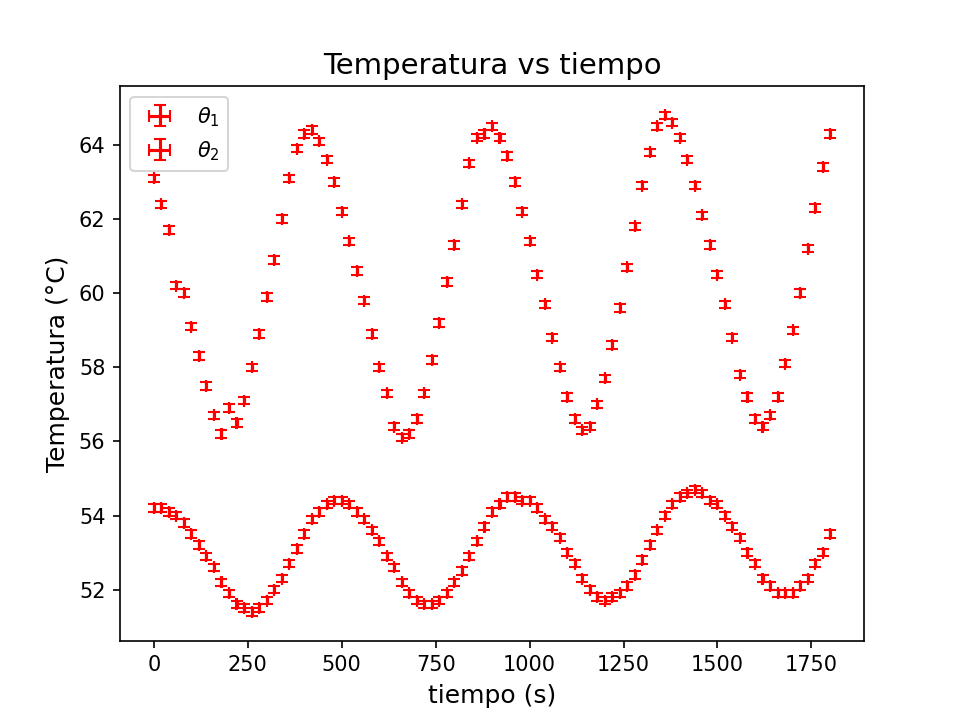
\includegraphics[width=0.8\textwidth]{grafica_temperatura.png}
    \caption{Oscilaciones de temperatura en función del tiempo en las dos posiciones de los sensores.}
    \label{fig:temp_plot}
\end{figure}

Los datos se ajustaron a un modelo sinusoidal utilizando Regresión Ortogonal de Distancia:
\begin{equation}
    \theta(t) = A + \text{Amp} \cdot \cos\left(\frac{2\pi}{\tau}t - \phi\right)
\end{equation}

Los resultados del ajuste, siguiendo la normativa GUM para cifras significativas, se resumen en la Tabla~\ref{tab:fit_results}.

\begin{table}[H]
    \centering
    \caption{Parámetros de ajuste para las oscilaciones térmicas en los sensores 1 y 2.}
    \label{tab:fit_results}
    \begin{tabular}{lrr}
        \toprule
        Parámetro & {Sensor 1 ($\theta_1$)} & {Sensor 2 ($\theta_2$)} \\
        \midrule
        Temp. media $A$ ($^\circ$C) & $53.110 \pm 0.018$ & $60.471 \pm 0.031$ \\
        Amplitud $Amp$ ($^\circ$C) & $1.399 \pm 0.025$ & $-3.978 \pm 0.044$ \\
        Periodo $\tau$ (s) & $475.8 \pm 1.3$ & $474.81 \pm 0.72$ \\
        Desfase $\phi$ (rad) & $0.201 \pm 0.037$ & $2.486 \pm 0.021$ \\
        \bottomrule
    \end{tabular}
\end{table}

\subsection{Parámetros físicos derivados}
A partir de la atenuación y el desfase, se calcularon los parámetros $m$ y $h$ para la distancia $d = (0.050 \pm 0.001)\,\mathrm{m}$. Estos parámetros se utilizaron posteriormente para determinar la difusividad térmica ($K_{exp}$) y la conductividad térmica experimental ($\lambda_{exp}$).

\begin{itemize}
    \item $m = (20.91 \pm 0.60)\,\mathrm{m^{-1}}$
    \item $h = (45.7 \pm 1.3)\,\mathrm{m^{-1}}$
    \item $K_{exp} = (16.75 \pm 0.81)\,\mathrm{m^2\,s^{-1}}$
    \item $\lambda_{exp} = (138.4 \pm 5.8)\,\mathrm{W\,m^{-1}\,K^{-1}}$
\end{itemize}

\section{Discusión}

El análisis de los datos experimentales registrados en el estado estacionario ha permitido ver con precisión el comportamiento ondulatorio del flujo de calor a lo largo de la barra de aluminio. A partir del ajuste, se han determinado unas amplitudes de oscilación térmica de $A_1 = 1.399 \pm 0.025$~$^\circ$C y $|A_2| = 3.978 \pm 0.044$~$^\circ$C. Ambos sensores registran un periodo de oscilación prácticamente idéntico ($\tau \approx 475$~s), lo que confirma que la frecuencia de excitación térmica se conserva durante la propagación.

Utilizando la distancia conocida entre los sensores ($d = 0.0500 \pm 0.0010$~m) y la diferencia de fase extraída de los ajustes, se han calculado los parámetros cinemáticos de la onda térmica. El coeficiente de atenuación obtenido es $m = 20.91 \pm 0.60$~m$^{-1}$, lo que demuestra la caída exponencial de la amplitud de la onda. Por otro lado, la constante de desfase calculada es $h = 45.7 \pm 1.3$~m$^{-1}$. 

A partir de estos parámetros ondulatorios, se ha deducido la conductividad térmica experimental del material, obteniendo un valor de $\lambda_{exp} = 138.4 \pm 5.8$~W$\cdot$m$^{-1}$K$^{-1}$. Al comparar este resultado con el valor teórico que tiene el aluminio a temperatura ambiente ($\lambda_{teo} \approx 237$~W$\cdot$m$^{-1}$K$^{-1}$), se observa un error significativo, siendo la o tenida un poco menos que la mitad de la teórica. Esta discrepancia, puede deberse al montaje experimental. 

En las ecuaciones del método que usamos asumimos un flujo de calor a través de una barra perfectamente aislada en su superficie lateral. Sin embargo, en el laboratorio, el dispositivo experimental puede no estar perfectamente aislado, permitiendo la entradad de aire. Esto quiere decir que existe una transferencia de calor no despreciable hacia el ambiente mediante mecanismos de convección natural y radiación térmica. Estas pérdidas provocan que la energía de la onda térmica se disipe más rápidamente que si únicamente operase el mecanismo de conducción interna. Por tanto, los resultados obtenidos son coherentes con las condiciones no ideales del contorno, demostrando la alta sensibilidad del método dinámico frente a las pérdidas de calor transversales.

\section{Conclusiones}
En conclusión, en esta práctica hemos determinado la conductividad térmica de una barra de aluminio. A través del estudio del estado estacionario, hemoes estudiado con éxito los fenómenos de propagación del calor en el aluminio: la amplitud térmica y el desfase entre dos sensores separados por una distancia conocida.

A partir del ajuste analítico riguroso de los datos experimentales, se aislaron los parámetros ondulatorios ($m$ y $h$) necesarios para deducir las propiedades térmicas del metal, culminando en un valor de conductividad experimental de $\lambda_{exp} = 138.4 \pm 5.8$~W$\cdot$m$^{-1}$K$^{-1}$.

Al comparar este resultado con el valor teórico (aproximadamente $237$~W$\cdot$m$^{-1}$K$^{-1}$), vemos claramente un error muy grande si lo comparamos con el obtenido experimenmentalmente. Pero esto no signfica que esté mal el experimento, es por la asunción de un aislamiento térmico perfecto. En el montaje real, la barra experimenta continuas pérdidas de calor hacia el ambiente circundante por convección y radiación. Estas transferencias provocan una caída bastante graned de la amplitud de onda. 

La práctica muestra lla transmisión de calor por ondas, y a la vez recalca la importancia de las condiciones experimentales a la hora de aplicar un modelo teórico a un sistema físico real que no es ideal y hace que la teoría pueda fallar.

\section{Cuestiones Teóricas}

En relación con las cuestiones teóricas planteadas en la práctica de laboratorio, estas son las respuestas a las preguntas:
\begin{itemize}
    \item \textbf{Q1:} El resultado analítico obtenido no depende de las unidades en las que se midan las amplitudes térmicas. El cálculo del coeficiente de atenuación, $m$, se basa en el logaritmo neperiano de ambas amplitudes, $\ln(A_2/A_1)$ \cite{guiones_pract}. Al tratarse de un cociente, cualquier factor de escala o conversión entre unidades de incremento de temperatura se cancela matemáticamente, al estar dividiendo dos cosas con las mismas unidades, manteniendo igual el resultado para todas las unidades en las que se ponga la amplitud.
    
    \item \textbf{Q2:} La incorporación de un ventilador en uno de los extremos del dispositivo tiene como objetivo principal forzar la convección térmica. Esto permite disipar el flujo de calor continuo que alcanza dicho extremo. Si el ventilador no estuviera colocado, el calor se iría acumulando, elevando la temperatura media de toda la barra metálica. En consecuencia, la temperatura global del sistema continuaría aumentando de forma indefinida, lo que impediría que las oscilaciones se estabilizaran en torno a un valor medio fijo. Sin alcanzar el régimen estacionario, resultaría matemáticamente imposible aplicar las ecuaciones teóricas usadas y no podríamos saber como es el comportamiento de la barra de alumino.
\end{itemize}

\section{Anexos}

\subsection{Datos Experimentales}
Todos los datos obtenidos durante el experimento se presentan en la Tabla~\ref{tab:raw_data}.

\begin{longtable}{rrrrrr}
    \caption{Datos experimentales de temperatura en función del tiempo.} \label{tab:raw_data} \\
    \toprule
    {$t$ (s)} & {$u_t$ (s)} & {$\theta_1$ (deg C)} & {$u_{\theta_1}$ (deg C)} & {$\theta_2$ (deg C)} & {$u_{\theta_2}$ (deg C)} \\
    \midrule
    \endfirsthead
    \multicolumn{6}{c}{{\bfseries \tablename\ \thetable{} -- Continuación de la página anterior}} \\
    \toprule
    {$t$ (s)} & {$u_t$ (s)} & {$\theta_1$ (deg C)} & {$u_{\theta_1}$ (deg C)} & {$\theta_2$ (deg C)} & {$u_{\theta_2}$ (deg C)} \\
    \midrule
    \endhead
    \midrule
    \multicolumn{6}{r}{{Continúa en la página siguiente}} \\
    \endfoot
    \bottomrule
    \endlastfoot
    0.00 & 0.10 & 54.20 & 0.10 & 63.10 & 0.10 \\
    20.00 & 0.10 & 54.20 & 0.10 & 62.40 & 0.10 \\
    40.00 & 0.10 & 54.10 & 0.10 & 61.70 & 0.10 \\
    60.00 & 0.10 & 54.00 & 0.10 & 60.20 & 0.10 \\
    80.00 & 0.10 & 53.80 & 0.10 & 60.00 & 0.10 \\
    100.00 & 0.10 & 53.50 & 0.10 & 59.10 & 0.10 \\
    120.00 & 0.10 & 53.20 & 0.10 & 58.30 & 0.10 \\
    140.00 & 0.10 & 52.90 & 0.10 & 57.50 & 0.10 \\
    160.00 & 0.10 & 52.60 & 0.10 & 56.70 & 0.10 \\
    180.00 & 0.10 & 52.20 & 0.10 & 56.20 & 0.10 \\
    200.00 & 0.10 & 51.90 & 0.10 & 56.90 & 0.10 \\
    220.00 & 0.10 & 51.60 & 0.10 & 56.50 & 0.10 \\
    240.00 & 0.10 & 51.50 & 0.10 & 57.10 & 0.10 \\
    260.00 & 0.10 & 51.40 & 0.10 & 58.00 & 0.10 \\
    280.00 & 0.10 & 51.50 & 0.10 & 58.90 & 0.10 \\
    300.00 & 0.10 & 51.70 & 0.10 & 59.90 & 0.10 \\
    320.00 & 0.10 & 52.00 & 0.10 & 60.90 & 0.10 \\
    340.00 & 0.10 & 52.30 & 0.10 & 62.00 & 0.10 \\
    360.00 & 0.10 & 52.70 & 0.10 & 63.10 & 0.10 \\
    380.00 & 0.10 & 53.10 & 0.10 & 63.90 & 0.10 \\
    400.00 & 0.10 & 53.50 & 0.10 & 64.30 & 0.10 \\
    420.00 & 0.10 & 53.90 & 0.10 & 64.40 & 0.10 \\
    440.00 & 0.10 & 54.10 & 0.10 & 64.10 & 0.10 \\
    460.00 & 0.10 & 54.30 & 0.10 & 63.60 & 0.10 \\
    480.00 & 0.10 & 54.40 & 0.10 & 63.00 & 0.10 \\
    500.00 & 0.10 & 54.40 & 0.10 & 62.20 & 0.10 \\
    520.00 & 0.10 & 54.30 & 0.10 & 61.40 & 0.10 \\
    540.00 & 0.10 & 54.10 & 0.10 & 60.60 & 0.10 \\
    560.00 & 0.10 & 53.90 & 0.10 & 59.80 & 0.10 \\
    580.00 & 0.10 & 53.60 & 0.10 & 58.90 & 0.10 \\
    600.00 & 0.10 & 53.30 & 0.10 & 58.00 & 0.10 \\
    620.00 & 0.10 & 52.90 & 0.10 & 57.30 & 0.10 \\
    640.00 & 0.10 & 52.60 & 0.10 & 56.40 & 0.10 \\
    660.00 & 0.10 & 52.20 & 0.10 & 56.10 & 0.10 \\
    680.00 & 0.10 & 51.90 & 0.10 & 56.20 & 0.10 \\
    700.00 & 0.10 & 51.70 & 0.10 & 56.60 & 0.10 \\
    720.00 & 0.10 & 51.60 & 0.10 & 57.30 & 0.10 \\
    740.00 & 0.10 & 51.60 & 0.10 & 58.20 & 0.10 \\
    760.00 & 0.10 & 51.70 & 0.10 & 59.20 & 0.10 \\
    780.00 & 0.10 & 51.90 & 0.10 & 60.30 & 0.10 \\
    800.00 & 0.10 & 52.20 & 0.10 & 61.30 & 0.10 \\
    820.00 & 0.10 & 52.50 & 0.10 & 62.40 & 0.10 \\
    840.00 & 0.10 & 52.90 & 0.10 & 63.50 & 0.10 \\
    860.00 & 0.10 & 53.30 & 0.10 & 64.20 & 0.10 \\
    880.00 & 0.10 & 53.70 & 0.10 & 64.30 & 0.10 \\
    900.00 & 0.10 & 54.10 & 0.10 & 64.50 & 0.10 \\
    920.00 & 0.10 & 54.30 & 0.10 & 64.20 & 0.10 \\
    940.00 & 0.10 & 54.50 & 0.10 & 63.70 & 0.10 \\
    960.00 & 0.10 & 54.50 & 0.10 & 63.00 & 0.10 \\
    980.00 & 0.10 & 54.40 & 0.10 & 62.20 & 0.10 \\
    1000.00 & 0.10 & 54.40 & 0.10 & 61.40 & 0.10 \\
    1020.00 & 0.10 & 54.20 & 0.10 & 60.50 & 0.10 \\
    1040.00 & 0.10 & 53.90 & 0.10 & 59.70 & 0.10 \\
    1060.00 & 0.10 & 53.70 & 0.10 & 58.80 & 0.10 \\
    1080.00 & 0.10 & 53.40 & 0.10 & 58.00 & 0.10 \\
    1100.00 & 0.10 & 53.00 & 0.10 & 57.20 & 0.10 \\
    1120.00 & 0.10 & 52.70 & 0.10 & 56.60 & 0.10 \\
    1140.00 & 0.10 & 52.30 & 0.10 & 56.30 & 0.10 \\
    1160.00 & 0.10 & 52.00 & 0.10 & 56.40 & 0.10 \\
    1180.00 & 0.10 & 51.80 & 0.10 & 57.00 & 0.10 \\
    1200.00 & 0.10 & 51.70 & 0.10 & 57.70 & 0.10 \\
    1220.00 & 0.10 & 51.80 & 0.10 & 58.60 & 0.10 \\
    1240.00 & 0.10 & 51.90 & 0.10 & 59.60 & 0.10 \\
    1260.00 & 0.10 & 52.10 & 0.10 & 60.70 & 0.10 \\
    1280.00 & 0.10 & 52.40 & 0.10 & 61.80 & 0.10 \\
    1300.00 & 0.10 & 52.80 & 0.10 & 62.90 & 0.10 \\
    1320.00 & 0.10 & 53.20 & 0.10 & 63.80 & 0.10 \\
    1340.00 & 0.10 & 53.60 & 0.10 & 64.50 & 0.10 \\
    1360.00 & 0.10 & 54.00 & 0.10 & 64.80 & 0.10 \\
    1380.00 & 0.10 & 54.30 & 0.10 & 64.60 & 0.10 \\
    1400.00 & 0.10 & 54.50 & 0.10 & 64.20 & 0.10 \\
    1420.00 & 0.10 & 54.60 & 0.10 & 63.60 & 0.10 \\
    1440.00 & 0.10 & 54.70 & 0.10 & 62.90 & 0.10 \\
    1460.00 & 0.10 & 54.60 & 0.10 & 62.10 & 0.10 \\
    1480.00 & 0.10 & 54.40 & 0.10 & 61.30 & 0.10 \\
    1500.00 & 0.10 & 54.30 & 0.10 & 60.50 & 0.10 \\
    1520.00 & 0.10 & 54.00 & 0.10 & 59.70 & 0.10 \\
    1540.00 & 0.10 & 53.70 & 0.10 & 58.80 & 0.10 \\
    1560.00 & 0.10 & 53.40 & 0.10 & 57.80 & 0.10 \\
    1580.00 & 0.10 & 53.00 & 0.10 & 57.20 & 0.10 \\
    1600.00 & 0.10 & 52.70 & 0.10 & 56.60 & 0.10 \\
    1620.00 & 0.10 & 52.30 & 0.10 & 56.40 & 0.10 \\
    1640.00 & 0.10 & 52.10 & 0.10 & 56.70 & 0.10 \\
    1660.00 & 0.10 & 51.90 & 0.10 & 57.20 & 0.10 \\
    1680.00 & 0.10 & 51.90 & 0.10 & 58.10 & 0.10 \\
    1700.00 & 0.10 & 51.90 & 0.10 & 59.00 & 0.10 \\
    1720.00 & 0.10 & 52.10 & 0.10 & 60.00 & 0.10 \\
    1740.00 & 0.10 & 52.30 & 0.10 & 61.20 & 0.10 \\
    1760.00 & 0.10 & 52.70 & 0.10 & 62.30 & 0.10 \\
    1780.00 & 0.10 & 53.00 & 0.10 & 63.40 & 0.10 \\
    1800.00 & 0.10 & 53.50 & 0.10 & 64.30 & 0.10 \\
\end{longtable}

\subsection{Incertidumbres}

En esta práctica se ha trabajado tanto con medidas directas como indirectas. A continuación se detalla el origen de la incertidumbre en cada magnitud.

\subsubsection*{Medidas directas}
Las medidas de temperatura ($\theta_1$, $\theta_2$), el tiempo ($t$) y la distancia entre termopares ($d$) son magnitudes obtenidas directamente de los instrumentos de laboratorio. 
\begin{itemize}
    \item La incertidumbre en el tiempo viene dada por la resolución del cronómetro o sistema de adquisición: $u_t = 0.1$~s.
    \item La incertidumbre de los termopares está determinada por la precisión del instrumento de medida digital: $u_{\theta} = 0.1$~$^\circ$C.
    \item La incertidumbre en la distancia se asume a partir del error de paralaje y la resolución de la regla graduada: $u_d = 0.001$~m.
\end{itemize}
Adicionalmente, las amplitudes ($A_1$, $A_2$), el periodo ($\tau$) y el desfase temporal ($\phi$) proceden del ajuste, por lo que su incertidumbre es el error estándar de los parámetros que lo da el algoritmo que hemos usado.

\subsubsection*{Medidas indirectas}
Para el cálculo de las variables físicas derivadas ($m$, $h$, difusividad $\lambda_{exp}$ y conductividad térmica $K_{exp}$) se ha empleado la ley de propagación cuadrática de incertidumbres:
\begin{equation}
    u_y = \sqrt{\sum_{i} \left( \frac{\partial y}{\partial x_i} u_{x_i} \right)^2}
\end{equation}

A continuación se muestran las expresiones analíticas de las derivadas parciales para cada magnitud y la fórmula final resultante:

\paragraph{1. Coeficiente de atenuación ($m$):}
Dada la expresión $m = \frac{1}{d} \ln\left(\frac{A_2}{A_1}\right)$, sus derivadas parciales son:
\begin{align}
    \frac{\partial m}{\partial A_1} &= -\frac{1}{A_1 d} \\
    \frac{\partial m}{\partial A_2} &= \frac{1}{A_2 d} \\
    \frac{\partial m}{\partial d} &= -\frac{1}{d^2} \ln\left(\frac{A_2}{A_1}\right)
\end{align}
Sustituyendo en la expresión general, la \textbf{fórmula final de la incertidumbre} es:
\begin{equation}
    u_m = \sqrt{ \left( -\frac{u_{A_1}}{A_1 d} \right)^2 + \left( \frac{u_{A_2}}{A_2 d} \right)^2 + \left( -\frac{1}{d^2} \ln\left(\frac{A_2}{A_1}\right) u_d \right)^2 }
\end{equation}

\paragraph{2. Constante de desfase ($h$):}
Sabiendo que $h = \frac{\phi}{d}$, las derivadas son:
\begin{align}
    \frac{\partial h}{\partial \phi} &= \frac{1}{d} \\
    \frac{\partial h}{\partial d} &= -\frac{\phi}{d^2}
\end{align}
Sustituyendo, la \textbf{fórmula final de la incertidumbre} es:
\begin{equation}
    u_h = \sqrt{ \left( \frac{u_{\phi}}{d} \right)^2 + \left( -\frac{\phi}{d^2} u_d \right)^2 }
\end{equation}

\paragraph{3. Difusividad térmica ($\lambda_{exp}$):}
A partir de $\lambda_{exp} = \frac{\omega}{2 m h}$ (donde $\omega = 2\pi / \tau$), las derivadas parciales resultan:
\begin{align}
    \frac{\partial \lambda_{exp}}{\partial \omega} &= \frac{1}{2 m h} \\
    \frac{\partial \lambda_{exp}}{\partial m} &= -\frac{\omega}{2 m^2 h} \\
    \frac{\partial \lambda_{exp}}{\partial h} &= -\frac{\omega}{2 m h^2}
\end{align}
\textit{Nota: La incertidumbre de la frecuencia angular se propaga como $u_{\omega} = \frac{2\pi}{\tau^2} u_{\tau}$.}

Sustituyendo, la \textbf{fórmula final de la incertidumbre} es:
\begin{equation}
    u_{\lambda_{exp}} = \sqrt{ \left( \frac{u_{\omega}}{2 m h} \right)^2 + \left( -\frac{\omega}{2 m^2 h} u_m \right)^2 + \left( -\frac{\omega}{2 m h^2} u_h \right)^2 }
\end{equation}

\paragraph{4. Conductividad térmica ($K_{exp}$):}
Asumiendo que la densidad ($\rho$) y el calor específico ($c$) del material se toman como valores tabulados exactos (es decir, sin incertidumbre apreciable frente a las medidas experimentales), la conductividad viene dada por $K_{exp} = \lambda_{exp} \rho c$. Su derivada parcial respecto a la única variable con error es:
\begin{align}
    \frac{\partial K_{exp}}{\partial \lambda_{exp}} &= \rho c
\end{align}

Sustituyendo en la expresión general de propagación cuadrática, la \textbf{fórmula final de la incertidumbre} es:
\begin{equation}
    u_{K_{exp}} = \sqrt{ \left( \rho c \cdot u_{\lambda_{exp}} \right)^2 }
\end{equation}


\newpage
\section{References}

\begin{thebibliography}{99}
    
    \bibitem{guiones_pract} Universidad de Granada (2026). \textit{Guiones de Prácticas de Física}. Disponible en: \url{https://pradogrado2526.ugr.es/pluginfile.php/710739/mod_resource/content/2/guiones_pract.pdf}
    
\end{thebibliography}

\end{document}
